                             %% ut-thesis.tex -- document template for graduate theses at UofT
%%
%% Copyright (c) 1998-2012 Francois Pitt <fpitt@cs.utoronto.ca>
%% last updated at 09:43 (EDT) on Fri  1 Jun 2012
%%
%% This work may be distributed and/or modified under the conditions of
%% the LaTeX Project Public License, either version 1.3c of this license
%% or (at your option) any later version.
%% The latest version of this license is in
%%     http://www.latex-project.org/lppl.txt
%% and version 1.3c or later is part of all distributions of LaTeX
%% version 2005/12/01 or later.
%%
%% This work has the LPPL maintenance status "maintained".
%%
%% The Current Maintainer of this work is
%% Francois Pitt <fpitt@cs.utoronto.ca>.
%%
%% This work consists of the files listed in the accompanying README.

%% SUMMARY OF FEATURES:
%%
%% All environments, commands, and options provided by the `ut-thesis'
%% class will be described below, at the point where they should appear
%% in the document.  See the file `ut-thesis.cls' for more details.
%%
%% To explicitly set the pagestyle of any blank page inserted with
%% \cleardoublepage, use one of \clearemptydoublepage,
%% \clearplaindoublepage, \clearthesisdoublepage, or
%% \clearstandarddoublepage (to use the style currently in effect).
%%
%% For single-spaced quotes or quotations, use the `longquote' and
%% `longquotation' environments.


%%%%%%%%%%%%         PREAMBLE         %%%%%%%%%%%%

%%  - Default settings format a final copy (single-sided, normal
%%    margins, one-and-a-half-spaced with single-spaced notes).
%%  - For a rough copy (double-sided, normal margins, double-spaced,
%%    with the word "DRAFT" printed at each corner of every page), use
%%    the `draft' option.
%%  - The default global line spacing can be changed with one of the
%%    options `singlespaced', `onehalfspaced', or `doublespaced'.
%%  - Footnotes and marginal notes are all single-spaced by default, but
%%    can be made to have the same spacing as the rest of the document
%%    by using the option `standardspacednotes'.
%%  - The size of the margins can be changed with one of the options:
%%     . `narrowmargins' (1 1/4" left, 3/4" others),
%%     . `normalmargins' (1 1/4" left, 1" others),
%%     . `widemargins' (1 1/4" all),
%%     . `extrawidemargins' (1 1/2" all).
%%  - The pagestyle of "cleared" pages (empty pages inserted in
%%    two-sided documents to put the next page on the right-hand side)
%%    can be set with one of the options `cleardoublepagestyleempty',
%%    `cleardoublepagestyleplain', or `cleardoublepagestylestandard'.
%%  - Any other standard option for the `report' document class can be
%%    used to override the default or draft settings (such as `10pt',
%%    `11pt', `12pt'), and standard LaTeX packages can be used to
%%    further customize the layout and/or formatting of the document.

%% *** Add any desired options. ***
\documentclass[doublespaced, 12pt]{ut-thesis}
\usepackage{natbib}
\usepackage{times}
\usepackage{url}
\usepackage{latexsym}
\usepackage{caption}
\usepackage{amsmath}

%
\usepackage{multirow}
\usepackage{subfig}
\usepackage{lipsum}                    
\usepackage{xargs}                     
\usepackage{graphicx}
\graphicspath{ {images/} }
\usepackage[pdftex,dvipsnames]{xcolor} 
\usepackage[colorinlistoftodos,prependcaption,textsize=tiny]{todonotes}
\newcommandx{\unsure}[2][1=]{\todo[linecolor=red,backgroundcolor=red!25,bordercolor=red,#1]{#2}}
\newcommandx{\change}[2][1=]{\todo[linecolor=blue,backgroundcolor=blue!25,bordercolor=blue,#1]{#2}}
\newcommandx{\info}[2][1=]{\todo[linecolor=OliveGreen,backgroundcolor=OliveGreen!25,bordercolor=OliveGreen,#1]{#2}}
\newcommandx{\improvement}[2][1=]{\todo[linecolor=Plum,backgroundcolor=Plum!25,bordercolor=Plum,#1]{#2}}
\newcommandx{\thiswillnotshow}[2][1=]{\todo[disable,#1]{#2}}

\newcommand{\tabref}[1]{Table \ref{#1}}
\newcommand{\figref}[1]{Figure \ref{#1}}
\newcommand{\secref}[1]{Section \ref{#1}}
\newcommand{\chapref}[1]{Chapter \ref{#1}}


\newcommand{\limit}[0]{\textrm{limit}}

%% *** Add \usepackage declarations here. ***
%% The standard packages `geometry' and `setspace' are already loaded by
%% `ut-thesis' -- see their documentation for details of the features
%% they provide.  In particular, you may use the \geometry command here
%% to adjust the margins if none of the ut-thesis options are suitable
%% (see the `geometry' package for details).  You may also use the
%% \setstretch command to set the line spacing to a value other than
%% single, one-and-a-half, or double spaced (see the `setspace' package
%% for details).


%%%%%%%%%%%%%%%%%%%%%%%%%%%%%%%%%%%%%%%%%%%%%%%%%%%%%%%%%%%%%%%%%%%%%%%%
%%                                                                    %%
%%                   ***   I M P O R T A N T   ***                    %%
%%                                                                    %%
%%  Fill in the following fields with the required information:       %%
%%   - \degree{...}       name of the degree obtained                 %%
%%   - \department{...}   name of the graduate department             %%
%%   - \gradyear{...}     year of graduation                          %%
%%   - \author{...}       name of the author                          %%
%%   - \title{...}        title of the thesis                         %%
%%%%%%%%%%%%%%%%%%%%%%%%%%%%%%%%%%%%%%%%%%%%%%%%%%%%%%%%%%%%%%%%%%%%%%%%

%% *** Change this example to appropriate values. ***
\degree{Master of Science}
\department{Computer Science}
\gradyear{2016}
\author{Priya Sidhaye}
\title{Examining Indicative Tweet Generation As An Extractive Summarization Problem}

%% *** NOTE ***
%% Put here all other formatting commands that belong in the preamble.
%% In particular, you should put all of your \newcommand's,
%% \newenvironment's, \newtheorem's, etc. (in other words, all the
%% global definitions that you will need throughout your thesis) in a
%% separate file and use "\input{filename}" to input it here.


%% *** Adjust the following settings as desired. ***

%% List only down to subsections in the table of contents;
%% 0=chapter, 1=section, 2=subsection, 3=subsubsection, etc.
\setcounter{tocdepth}{2}

%% Make each page fill up the entire page.
\flushbottom


%%%%%%%%%%%%      MAIN  DOCUMENT      %%%%%%%%%%%%

\begin{document}

%% This sets the page style and numbering for preliminary sections.
\begin{preliminary}

%% This generates the title page from the information given above.
\maketitle

%% There should be NOTHING between the title page and abstract.
%% However, if your document is two-sided and you want the abstract
%% _not_ to appear on the back of the title page, then uncomment the
%% following line.
%\cleardoublepage

%% This generates the abstract page, with the line spacing adjusted
%% according to SGS guidelines.
\begin{abstract}
%% *** Put your Abstract here. ***
%% (At most 150 words for M.Sc. or 350 words for Ph.D.)
Social media such as Twitter have become an important method of communication, with potential opportunities for NLG to facilitate the generation of social media content. We focus on the generation of \emph{indicative tweets} that contain a link to an external web page. While it is natural and tempting to view the linked web page as the source text from which the tweet is generated in an extractive summarization setting, it is unclear to what extent actual indicative tweets behave like extractive summaries. We collect a corpus of indicative tweets with their associated articles and investigate to what extent they can be derived from the articles using extractive methods. We also consider the impact of the formality and genre of the article.

With the aim of finding the possible factors that influence the probability of the tweet being a summarization of the article, we conduct further studies to detect the function of the tweet. The results that are significant show a positive correlation between the extractiveness and informativeness of the tweet. In the analysis of these questions, we have also generated a dataset of various tweets categorized by their subjects and  spanning broad areas of public interest, along with text in newspaper articles linked to by these tweets. The judgements provided by the human evaluators in our user study are also added to the data to make a human-tagged dataset for identifying functions of tweets.

Our results demonstrate the limits of viewing indicative tweet generation as extractive summarization, and point to the need for the development of a methodology for tweet generation that is sensitive to genre-specific issues.

\end{abstract}

\begin{abstract}
french abstract
\end{abstract}

% \chapter*{Acknowledgements}
\begin{acknowledgements}

I would like to thank my supervisor, Jackie Cheung, who has been a teacher and advisor and helped me not just by guiding my thesis, but also by creating a fun research group that I am proud to be a part of.

I would like to thank Prof. Joelle Pineau for putting me in touch with Jackie for my thesis, Jad Kabbara for helping me translate my abstract to French, and everyone in the very large Reasoning and Learning lab family.

I would also like to thank my parents, my family and friends who have been a constant emotional support system, to be always relied upon.

I would like to thank Julian Brooke for providing the formality lexicon used in part of this study, and Prof. Derek Ruths for agreeing to be the external reviewer of the thesis.

Last but not the least, I thank the McGill University community for a wonderful experience and for teaching me a thing or two beyond the subjects I came here to study.  
\end{acknowledgements}

%% Anything placed between the abstract and table of contents will
%% appear on a separate page since the abstract ends with \newpage and
%% the table of contents starts with \clearpage.  Use \cleardoublepage
%% for anything that you want to appear on a right-hand page.

%% This generates a "dedication" section, if needed
%% (uncomment to have it appear in the document).
%\begin{dedication}
%% *** Put your Dedication here. ***
%\end{dedication}

%% The `dedication' and `acknowledgements' sections do not create new
%% pages so if you want the two sections to appear on separate pages,
%% you should put an explicit \newpage between them.

%% This generates an "acknowledgements" section, if needed
%% (uncomment to have it appear in the document).
%\begin{acknowledgements}
%% *** Put your Acknowledgements here. ***
%\end{acknowledgements}

%% This generates the Table of Contents (on a separate page).
\tableofcontents

%% This generates the List of Tables (on a separate page), if needed
%% (uncomment to have it appear in the document).
\listoftables

%% This generates the List of Figures (on a separate page), if needed
%% (uncomment to have it appear in the document).
\listoffigures

%% You can add commands here to generate any other material that belongs
%% in the head matter (for example, List of Plates, Index of Symbols, or
%% List of Appendices).

%% End of the preliminary sections: reset page style and numbering.
\end{preliminary}


%%%%%%%%%%%%%%%%%%%%%%%%%%%%%%%%%%%%%%%%%%%%%%%%%%%%%%%%%%%%%%%%%%%%%%%%
%%  Put your Chapters here; the easiest way to do this is to keep     %%
%%  each chapter in a separate file and `\include' all the files.     %%
%%  Each chapter file should start with "\chapter{ChapterName}".      %%
%%  Note that using `\include' instead of `\input' will make each     %%
%%  chapter start on a new page, and allow you to format only parts   %%
%%  of your thesis at a time by using `\includeonly'.                 %%
%%%%%%%%%%%%%%%%%%%%%%%%%%%%%%%%%%%%%%%%%%%%%%%%%%%%%%%%%%%%%%%%%%%%%%%%

%% *** Include chapter files here. ***
\chapter{Introduction}
\label{chap:intro}

Social media comprise a large part of our lives, with various outlets providing a platform for sharing thoughts, news, images and videos. With the rise in popularity of social media, message broadcasting sites such as Twitter and other microblogging services have become an important means of communication, with an estimated 500 million tweets being written every day\footnote{https://about.twitter.com/company}. In addition to individual users, various organizations and public figures such as newspapers, government officials and entertainers have established themselves on social media in order to disseminate information or promote their products. Social media thus provide an incredibly dense and varied source of data, originating from people and organizations all over the world.

Following the prolific increase in the use of social media, there has been an increase in the number of studies in natural language processing using the sources of data social media provide. Specifically for Twitter, these include areas such as tweet parsing \citep{ritter2011named, kong-etal-2014}, text normalization \citep{han2011lexical, kaufmann2010syntactic}, tweet POS tagging \citep{gimpel2011part, owoputi-etal-2013}, sentiment analysis of tweets \citep{kouloumpis2011twitter, mohammad2013nrc}, event summarization \citep{chakrabarti2011event, nichols2012summarizing}, identifying bot behaviours \citep{chu2012detecting} and inferring things like political views of individuals \citep{mohammad2013identifying}. While this progress in the development of Twitter-specific POS taggers, parsers, and other tweet understanding tools is encouraging, there has been little work on methods for \textit{generating tweets}. Methods to generate tweets would be beneficial to users and organizations for the purposes of advertisement, education, or even entertainment. Examples of such uses include generating tweets that advertise products or services based on some online review articles, or notifying users of closure of roads because of construction work by local governments.

% , despite the utility this would have for users and organizations, for purposes of advertisement, education, or even entertainment. 

In this thesis, we study the generation of the particular class of tweets that contain a link to an external web page that is composed primarily of text. Given the short length of a tweet, the presence of a URL in the tweet is a strong signal that the tweet is functioning to help Twitter users decide whether to read the full article. We call this class of tweets \emph{indicative tweets}, since they act as indicative summaries of the articles they are being linked to. Indicative tweets represent a large subset of tweets overall, constituting more than half (53.4\%) of the tweets in a data set that we collected in \chapref{chap:data}. Generating indicative tweets would appear to be a feasible problem to solve using current methods in text summarization, such as extractive summarization, because there is a clear source of input from which a tweet could be generated. 

% It should be noted that a tweet being indicative does not preclude it from also providing a critical evaluation of the linked article.

There has in fact been some work along these lines, within the framework of extractive summarization. \cite{lofi2012iparticipate} describe a system to generate tweets from local government records through keyword generation. However, they do not provide a formal evaluation for their proposed system.

\cite{lloret2013towards} compare various extractive summarization algorithms applied on Twitter data to generate tweets from documents. They compare the overlap between system-generated and user-generated tweets using ROUGE 
\citep{lin2004rouge}, a recall-based evaluation metric for summarization, and achieve some success in generating tweets based on ROUGE scores. Unfortunately, they also show that there is little correlation between ROUGE scores and the perceived quality of the tweets when rated by human users for indicativeness and interest. An \textit{indicative} text is one that aims to point to or generate interest about something. Hence the \textit{indicativeness} of a tweet can be defined as a measure of how strongly it points to the article. More discussion about these studies is done in \chapref{chap:background}.

Beyond issues of evaluation measures, it is also unclear whether extraction is the strategy employed by human tweeters. One of the original motivations behind extractive summarization for news text was the observation that human summary writers tended to extract snippets of key phrases from the source text \citep{mani-2001}.  And while it may be true that an automatic tweet generation system need not necessarily follow the same approach to writing as human tweeters, it is still necessary to know what proportion of tweets could be accounted for in an extractive summarization paradigm. More scrutiny is required to determine whether methods and evaluation schemes from extractive summarization can be adopted for the purpose of producing indicative tweets and is one of the primary aims of this thesis. With indicative tweets, an additional issue arises in that the genre of the source text is not constrained; for example it may be a news article or an informal blog post or an advertisement. This genre of the source text may be vastly different from the desired formality of tweet itself, and thus, a genre-appropriate extract may not be available. 


\paragraph{Contributions}
We begin to address the above issues through a study that examines to what extent tweet generation can be viewed as an extractive summarization problem. We extracted a dataset of indicative tweets containing a link to an external article, including the documents linked to by the tweets. We used this data and applied unigram, bigram and LCS (longest common subsequence) matching techniques inspired by ROUGE to determine what proportion of tweets can be found in the linked article.  This measure can also be defined as \emph{extractiveness} of the tweet, or the degree to which the tweet has been extracted from the article. Even with the permissive unigram match measure, we find that well under half of the tweet can be found in the linked article. We also use stylistic analysis on the articles to examine the role that genre differences between the source text and the target tweet play and if genre can give an indication for whether the tweet can be extracted. We find that tweets are extracted from articles with higher formality to a greater extent than ones with lower formality. 

We further conducted studies to identify functions for the tweets with respect to the articles. The data extracted from Twitter was presented to workers on a crowdsourcing website, to ask whether the tweets were indicative or informative. \textit{Informative} tweets are the ones that convey some information from the article, and \textit{informativeness} is defined as the degree to which the information from the article is conveyed in the tweet. We found a link between whether the tweet was deemed informative, and the degree to which a tweet has been extracted from the article, offering a better view of our ROUGE-inspired analysis methods detailed in \chapref{chap:analysis} and when they can be used for generating tweets. As a result, this dataset tagged by human evaluators has been generated and should be useful in further studies for identifying functions of tweets. 

Overall, our results point to the need for the development of a methodology for indicative tweet generation, rather than to expropriate the extractive summarization paradigm that was developed mostly on news text. Such a methodology will ideally be sensitive to stylistic factors as well as the underlying intent of the tweet.

\paragraph{Chapter Outline} \chapref{chap:background} contains the discussion on various related studies. The process of collecting the dataset is detailed in \chapref{chap:data}. \chapref{chap:analysis} contains the analyses performed on the dataset we collected. \chapref{chap:user} details the process of designing and executing the user study based on our data and analysis of the input from the workers. Finally, \chapref{chap:conclusion} contains the conclusions drawn from our the discussion of results in \chapref{chap:analysis} and \chapref{chap:user}.

Portions of \chapref{chap:intro}, \chapref{chap:data} and \chapref{chap:analysis} were published as part of the conference paper \cite{sidhayeindicative}. The contribution of the co-author was that of a thesis supervisor. 


\chapter{Background and Related Work}
\label{chap:background}

This chapter contains the literature survey and the background for the thesis. Background on various concepts used in the thesis alongwith numerous related studies, especially on Twitter data are then discussed.


\section{Summarization}

Summarization is the task of condensing the original text document while retaining as much of the important information as possible. Other goals include readability of the generated summary and coherence. The two main approaches for automatic text summarization are \textit{extractive} and \textit{abstractive} summarization. Extractive summarization uses the technique of extract and rearrange. \cite{nenkova2012survey} describe the components in extractive summarization techniques as building an internal representation of the important parts of the text, ranking these in the order of importance/time etc and then selecting a suitable list of these sentences to eventually form the summary. In phrase-level summarization, smoothing techniques may be used to generate readable texts. Sentence-level summarization techniques tend do be inherently more cohesive since sentences are directly picked out, however, sentence compression techniques can be used to reduce the size of the summaries. Even after using smoothing techniques to generate readable text, the summaries tend to be incoherent and hard to read. \figref{fig:extractive} shows an example of extractive summarization where a couple of sentences from the article have been picked to show in the the thumbnail for an article.

\begin{figure}[!htbp]
\centering
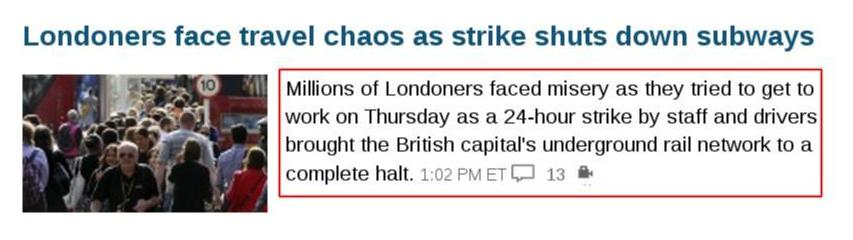
\includegraphics[width=\textwidth, height=4.5cm]{extractive}
\caption{Example of extractive summarization.}
\label{fig:extractive}
\end{figure}


The second approach is that of abstractive summarization. This is a text-to-text generation approach that aims at keeping the content or meaning of the text the same while condensing the text or generalizing it. As a rule, abstractive summarization requires world knowledge and is a much more difficult problem to solve. In fact, it is a rather large challenge and current summarization techniques concentrate on improving results from extractive summarization. \figref{fig:abstractive} shows the same thumbnail for a news article. However, the title of the article is an abstractive summary that is a generalization of the events described, carefully omitting details yet leaving the overall meaning of the event untouched.

\begin{figure}[!htbp]
\centering
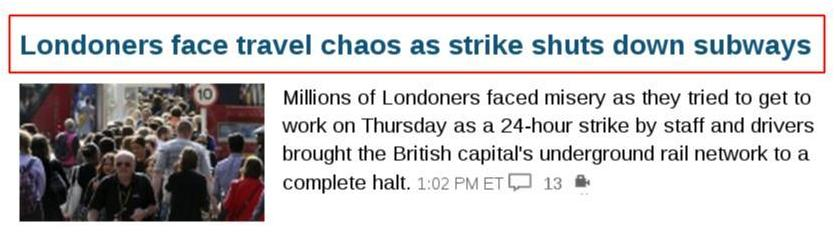
\includegraphics[width=\textwidth, height=4.5cm]{abstractive}
\caption{Example of abstractive summarization.}
\label{fig:abstractive}
\end{figure}

The limits of extractive summarization have been studied by \cite{he2000comparing}. They compare user preferences for various types of summaries of an audio-visual presentation. They demonstrate that the most preferred method of summarization is highlights and notes provided by the author, rather than transcripts or slides from the presentation. \cite{conroy2006topic} computed an oracle ROUGE score to investigate the same issue of the limits of extraction for news text. The oracle score is based on the maximum likelihood probability of words occurring in model summaries and is in turn used to generate summaries that perform better than any extracted and also human-generated summaries.

\subsection{ROUGE: Evaluation measure for Text Summarization}

ROUGE is an evaluation measure popularly used for evaluating quality of summaries and was proposed by \cite{lin-2004}. It measures the quality of the summary by comparing the output of the system being tested against a set of gold standard summaries. The intuition is that if the generated summary has enough in common with a set of human-written summaries, then it can be judged as a good summary. The different types of comparisons calculated are the unigram, bigram, trigram and least common subsequence(ROUGE-1,2,3 and L respectively). A set of gold standard summaries are used to encompass the number of possibilities while generating summaries. 

\begin{equation}
ROUGE-N = \frac{\sum\limits_{S \in \{Reference Summaries\}} \sum\limits_{gram_n \in S} Count_{match}(gram_n)}{\sum\limits_{S \in \{Reference Summaries\}} \sum\limits_{gram_n \in S} Count(gram_n)}
\end{equation}

The equation as described by \cite{lin2004looking} shows the calculation of the ROUGE-N score, where $n$ is the length of the n-gram, and $Count_{match}$ is the length of the matched n-grams in the summary and the reference summaries.

The use of multiple gold standard summaries gives rise to a subjective evaluation metric where the quality of the evaluation is dependent on the quality and number of the gold standard summaries. ROUGE also does not calculate take into account whether the summary is fluent or coherent. However, it is useful in the extractive text summarization systems where content retention needs to be judged since it uses n-gram co-occurrence statistics.

% \section{Stylistics}
%\change{remove this and put it in the formality part}
% Stylistics is referred to the characteristics of text that can be extracted from it that do not relate to the meaning of the text. Common examples of these include textual statistics such as length of sentences and words, parts of speech, function words etc. and finds applications in authorship attribution, semantic analysis, personality typing and so on. Studies on building lexicons for formality have been conducted and are discussed further later \chapref{chap:analysis}.

\section{Studies based on Twitter data}

There have been studies on a number of different issues related to Twitter data, including classifying tweets and sentiment analysis of tweets. \cite{ghosh2011entropy} classified the retweeting activity of users based on time intervals between retweets of a single user and frequency of retweets from unique users. 'Retweet' here means the occurrence of the same URL in a different tweet. The study was able to classify the retweeting as automatic or robotic retweeting, campaigns, news, blogs and so on, based on the time-interval and user-frequency distributions. In another study, \cite{chen2012extracting} were able to extract sentiment expressions from a corpus of tweets including both formal words and informal slang that bear sentiment.

Other studies using Twitter data include \cite{o2010tweetmotif}, who use topic summarization for a given search for better browsing. \cite{chakrabarti2011event} generate an event summary by learning about the event using a Hidden Markov Model over the tweets describing it. \cite{wang2014socially} generate a coherent event summary by treating summarization as an optimization problem for topic cohesion. \cite{inouye2011comparing} compare multiple summarization techniques to generate a summary of multi-post blogs on Twitter. \cite{wei2014utilizing} use tweets to help in generating better summaries of news articles.

% detailed analysis of this paper
As described in \chapref{chap:intro}, we analyze tweet generation using measures inspired by extractive summarization evaluation. There has been one study comparing different text summarization techniques for tweet generation by \cite{lloret2013towards}. Summarization systems were used to generate sentences lesser than 140 characters in length by summarizing documents, which could then be taken to be tweets. The system-generated tweets were evaluated using ROUGE measures \cite{lin2004rouge}. The ROUGE-1, ROUGE-2 and ROUGE-L measures were used, and a human-written reference tweet was taken to be the gold standard. %ROUGE has been known to work better when multiple reference summaries are used and is not meant to be used at the sentence level. This study uses ROUGE with a single reference summary, which is the reference tweet. However, given the size of a tweet, it can be argued that while generating a reference tweet from a single document, it is difficult to generate multiple reference tweets with largely varying content. \unsure{Is this reasoning okay?}

These studies show that extractive summarization algorithms may not generate good quality summaries despite giving high ROUGE evaluation scores. \cite{cheung2013towards} show that for the news genre, extractive summarization systems that are optimized for \textit{centrality}---that is, getting the core parts of the text into the summary---cannot perform well when compared to model summaries, since the model summaries are abstracted from the document to a large extent.



\chapter{Data Extraction and Preprocessing}
\label{chap:data}

This chapter discusses the collection of data for the thesis. The choice twitter for data extraction is discussed, along with the methods used for extracting the data. Then, the preprocessing done on the data is described. 


\section{Using Twitter for Data Extraction}

As mentioned earlier, there have been numerous studies that used data from the public Twitter feeds. However, none of the datasets in those studies focused on tweets and related articles linked to these tweets. The dataset of \cite{lloret2013towards} is an exception, as it contains tweets and the news articles they link to, but it only contains 200 English tweet-article pairs. \cite{wei2014utilizing} also constructed a dataset that contains both tweets and articles linked through them, but this data only deals with news text, and does not contain the variety of topics we wanted in the data. We therefore chose to build our own dataset. This section describes extraction, cleaning and other preprocessing of the data.

\section{Extracting Data}

Data was extracted from Twitter using the Twitter REST API using 51 search terms, or ‘hashtags’. These hashtags were chosen from a range of topics including pop culture,  international summit meetings discussing political issues, lawsuits and trials, social issues and health care issues. All these hashtags were ‘trending’ (being tweeted about at a high rate) at the time of extraction of the data. To get a broader sample, the data was extracted over the course of 15 days in November, 2014, which gave us multiple news stories to choose from for the search terms. The search terms were chosen so that there would be broad representation in terms of various stylistic properties of text like formality, subjectivity, etc. For example, searches related to politics would be more formal, while those related to films would be informal, and would also have a lot more opinion pieces about them. A few examples of the search terms and their distribution in genre are shown in \tabref{tab:searchterms}.

We extracted about 30,000 tweets, of which more than half, or around 16,000, contained URLs to an external news article, photo on photo sharing sites, or video. The hashtags were chosen to maximise the number of articles related to the tweets. Many topics that were chosen were being tweeted about by news agencies and other popular news sources.

\begin{table}[htbp]
\centering
\begin{tabular}{|l|l|}
\hline
\multicolumn{1}{|c|}{Politics}                                                       & \multicolumn{1}{c|}{Science \& Technology}                                               \\ \hline
\begin{tabular}[c]{@{}l@{}}\#apec2014\\ \#G20\\ \#oscarpistorius \\ \end{tabular}        & \begin{tabular}[c]{@{}l@{}}\#rosetta\\ \#lollipop\\ \#mangalayan\end{tabular}            \\ \hline
\multicolumn{1}{|c|}{Events}                                                         & \multicolumn{1}{c|}{Films and Pop culture}                                               \\ \hline
\begin{tabular}[c]{@{}l@{}}\#haiyan\\ \#memorialday\\ \#ottawashootings\end{tabular} & \begin{tabular}[c]{@{}l@{}}\#TaylorSwift\\ \#theforceawakens\\ \#johnoliver\end{tabular} \\ \hline
\multicolumn{1}{|c|}{International}                                                  & \multicolumn{1}{c|}{Sports}                                                              \\ \hline
\begin{tabular}[c]{@{}l@{}}\#berlinwall\\ \#ebola\\ \#erdogan\end{tabular}           & \begin{tabular}[c]{@{}l@{}}\#ausvssa\\ \#playingitmyway\\ \#nycmarathon\end{tabular}     \\ \hline
\end{tabular}
% \bigskip
\captionof{table}{Examples of the hashtags used for extraction, grouped into various categories.}
\label{tab:searchterms}
\end{table}

The data from the tweets was cleaned by removing the tweets that were not in English as well as the retweets; i.e., re-publications of a tweet by a different user.

We deduplicated the 16,000 extracted URLs into 6,003 unique addressed, then extracted and preprocessed their contents. The \texttt{newspaper} package\footnote{https://pypi.python.org/pypi/newspaper} was used to extract article text and the title from the web page. Since we are interested in text articles that can serve as the source text for summarization algorithms, we needed to remove photos and video links such as those from Instagram and YouTube. To do so, we removed those links that contained fewer than a threshold of 150 words. After this preprocessing, the number of useful articles was reduced from 6003 to 3066. There were some further tweet-article pairs where the text of the tweets was identical, these were removed by further preprocessing and the number of unique tweet-article pairs came down to 2471. 

The final version of the data consists of tweets along with other information about the tweet, such as links to articles, hashtags, time of publication, etc. We also retain the linked article text and preprocessed it using the CoreNLP toolkit \cite{manning2014stanford}. This includes the URL itself and the text extracted from the article, as well as some extracted information such as sentence boundaries, POS tags for tokens, parse trees and dependency trees. These annotations are used later during our analysis in \chapref{chap:analysis}. \tabref{tab:ex1} shows an example of an entry in the dataset.

A URL could have been tweeted through multiple tweets, all the ids of these tweets are linked to the same URL. It should be noted that the tweet to article dataset contains only the articles that are significantly long texts about the subject with a title, and contain no advertisements, other languages, or links to images or videos. 


\begin{table}[htbp]
\centering
\begin{tabular}{|p{0.1\linewidth}|p{0.8\linewidth}|}
\hline
Tweet & `\#RiggsReport: \#CA as the \#ElectionNight exception. Voters rewarded \#GOP nationally, but not in the \#GoldenState. http://t.co/K542wvSNVz' \\ \hline
Title & `The Riggs Report: California as the Election Night exception'                                                                                 \\ \hline
Text  & `When the dust settled on Election Night last week...'                                                                                         \\ \hline
\end{tabular}
\captionof{table}{Example of a tweet, title of the article and the text.}
\label{tab:ex1}
\end{table}


\chapter{Analysis}
\label{chap:analysis}

We now describe the analyses we performed on the data in this chapter. The chapter begins by discussing the ways we arrived at the calculations made on the data, the details of how these tasks were performed using the data described in \chapref{chap:data} and then goes on the discuss the results and the consequent conclusions derived from the results.

Our goal is to investigate what proportion of the indicative tweets that we extracted can be found in the articles that they link to, in order to determine whether indicative tweet generation can be viewed as an extractive summarization problem. \tabref{tab:noextract} gives an example of data where the tweet that was shared about the article does not come directly from the article text, while \tabref{tab:extract} shows a tweet that was almost entirely extracted from the text of the article, but changed a little for the purpose of readability.

\begin{table}[!htbp]
\centering
\begin{tabular}{|p{0.1\linewidth}|p{0.8\linewidth}|}
\hline
Tweet &  Are \#Airlines doing enough with \#Ebola? http://t.co/XExWwxmjnk \#travel \\ \hline
Title &  Could shortsighted airline refund policies lead to an outbreak? \\  \hline
Text  &  The deadly Ebola virus has arrived in the United States just in time for the holiday travel season, carrying fear and uncertainty with it... \\ \hline
\end{tabular}
\captionof{table}{Example of a tweet, title of the article and the text when tweet cannot be extracted from text.}
\label{tab:noextract}
\end{table}

\begin{table}[!htbp]
\centering
\begin{tabular}{|p{0.1\linewidth}|p{0.8\linewidth}|}
\hline
Tweet & Officer \textbf{Wilson will be returned to active duty if no indictment}, says \#Ferguson Police \textbf{Chief} http://t.co/zrRIBxMUYJ  \\ \hline
Title & Jackson clarifies comments on Wilson's future status \\ \hline
Text  & ...\textbf{Chief} Jackson said if the grand jury does \textbf{not indict Wilson}, he \textbf{will} immediately \textbf{return to active duty}.... \\ \hline
\end{tabular}
\captionof{table}{Example of a tweet, title of the article and the text when tweet can be extracted from text. The matched portions of the tweet and article are in bold.}
\label{tab:extract}
\end{table}

We first compute the proportion of tweets that can be recovered directly from the article in its entirety (\secref{sec:exact-match}). Then, we calculate the degree of overlap in terms of unigrams and bigrams between the tweet and the text of the document (Sections \ref{sec:unigrams}, \ref{sec:bigrams}). 

In addition, we consider locality within the article when computing the overlap. For the unigram analysis, we performed a variant of the analysis, in which we computed the overlap within three-sentence windows in the source article (\secref{sec:window}). We also compute the least common subsequences between the tweet and the document (\secref{sec:lcs}). This was done to investigate whether sentence compression techniques could be applied to local context windows to generate the tweet.

These calculations are analogous to the ROUGE-1, -2 and -L style calculations. These results give an indication of the degree to which the tweet is extracted from the document text. 

For all these analyses, the stop words have been eliminated from the tweet as well as the document, so that only the informative words are taken into consideration. The comparisons were made without lemmatization or stemming, to adhere closely to existing work in extractive summarization, where the only modifications to the source text are removing discourse cue words or removing words by sentence compression techniques. The hashtags, references (@) and URLs from the tweets were all removed for analysis.

\section {Exact Match Calculations}
\label{sec:exact-match}
We first checked for a complete substring match of the tweet in the text. Out of the 2471 unique instances of tweet and article pairs, a complete match was found only 23 times. In 9 cases out of these, the tweet text matched the title of the article, which our preprocessing tool did not correctly separate from the body of the article. In the other cases, the text of the tweet appears in its entirety inside the body of the article. This suggests that the user chose the sentence that either seemed to be the most conclusive contribution of the article, or expressed the opinion of the user to be tweeted. An example for this is detailed in \tabref{tab:fullextract}.

Apart from the 9 times where the tweet was matched with title in the article, we also checked to see if the tweet text matched with the article titles that were separately extracted by the \texttt{newspaper} package in order to determine if tweets could be generated using the headline generation methods. We found that it did not match with the titles. However, even though there are no exact matches, there might still be matches where the tweet is a slight modification of the headline of the article, and can be measured using a partial match measure.

\begin{table}[!htbp]
\centering
\begin{tabular}{|p{0.1\linewidth}|p{0.8\linewidth}|}
\hline
Tweet &  @PNHP: \textbf{6. Renounce punitive and counterproductive measures such as “sealing the borders,”} http://t.co/LRLS2MhPRE \#Ebola \\ \hline
Title & Physicians for a National Health Program \\  \hline
Text  & As health professionals and trainees, we call on President Obama to take the following immediate steps to address the Ebola crisis... \textbf{6. Renounce punitive and counterproductive measures such as “sealing the borders,”} and take steps to address the... \\ \hline
\end{tabular}
\captionof{table}{Example where tweet is extracted as is from the text, matched portion in bold.}
\label{tab:fullextract}
\end{table}


\begin{figure}[!htbp]
\centering
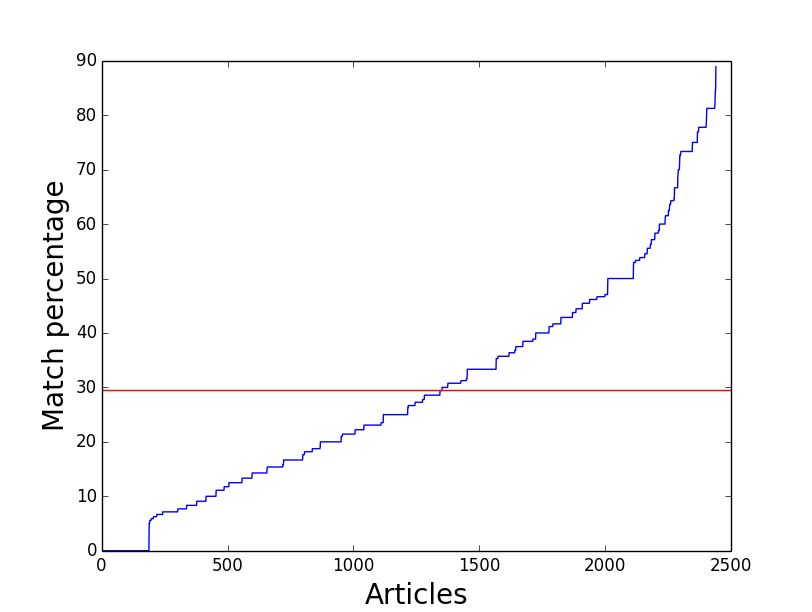
\includegraphics[width=0.7\textwidth, height=9cm]{unigrammatch}
\caption[Unigram matching percentages]{Distribution of unigram match percentage over unique tweets and articles. The mean is 29.53\%, indicated by the red horizontal line, with a standard deviation of 20.2\%}
\label{fig:unigrammatch}
\end{figure}


\begin{figure}[!htbp]
\centering
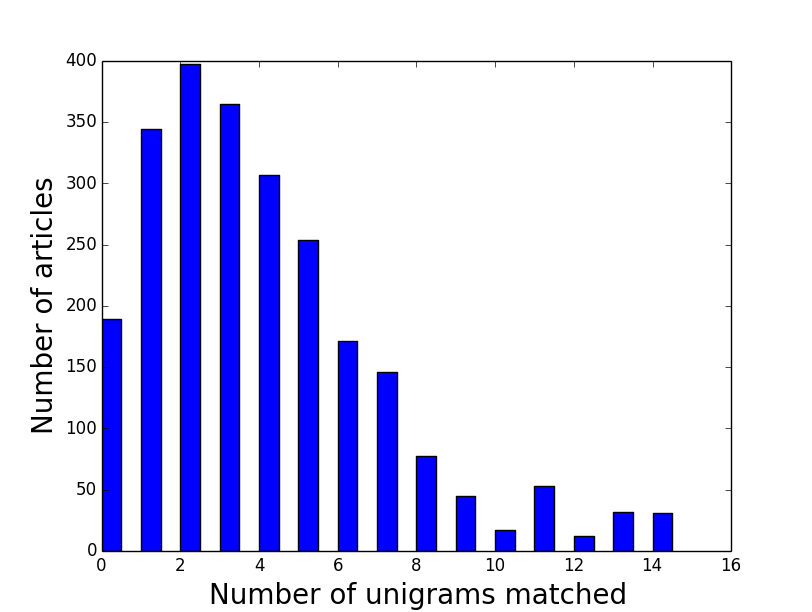
\includegraphics[width=0.7\textwidth, height=9cm]{num_unigrams}
\caption[Histogram for number of unigrams matched]{Histogram of number of unique tweet-article pairs vs number of unigrams matched. The mean number of unigrams matched per tweet-article pair is 3.9.}
\label{fig:num_unigrams}
\end{figure}


\section{Percentage Match for Unigrams}
\label{sec:unigrams}

Next, we did a percentage match with the text of the article. This was a bag-of-words check using unigram overlap between the tweet and the document. Let $\textit{unigrams}(x)$ be the set of unigrams for some text $x$, then $u$, the percentage of matching unigrams found between a given tweet, $t$ and a given article, $a$, can be defined as  

\begin{equation}
u = \frac{| \textit{unigrams}(t) \cap \textit{unigrams}(a) |}{| \textit{unigrams}(t) |} * 100
\end{equation}

\figref{fig:unigrammatch} shows the percentage of matches in the tweet and the article text as compared to the number of unigrams in the tweet. The mean match percentage is 29.53\% and standard deviation is 20.2\%. The mean of this distribution shows that the number of matched unigrams from a tweet in the article are fairly low. \figref{fig:num_unigrams} shows the number of articles with a certain number of matching unigrams. The graph shows that the most common number of unigrams matched was 2. The number of articles with higher unigrams matched goes on decreasing. The slight rise at the end - more than 10 matched unigrams - is accounted for by the completely matched tweets described above.

\begin{figure}[!htbp]
\centering
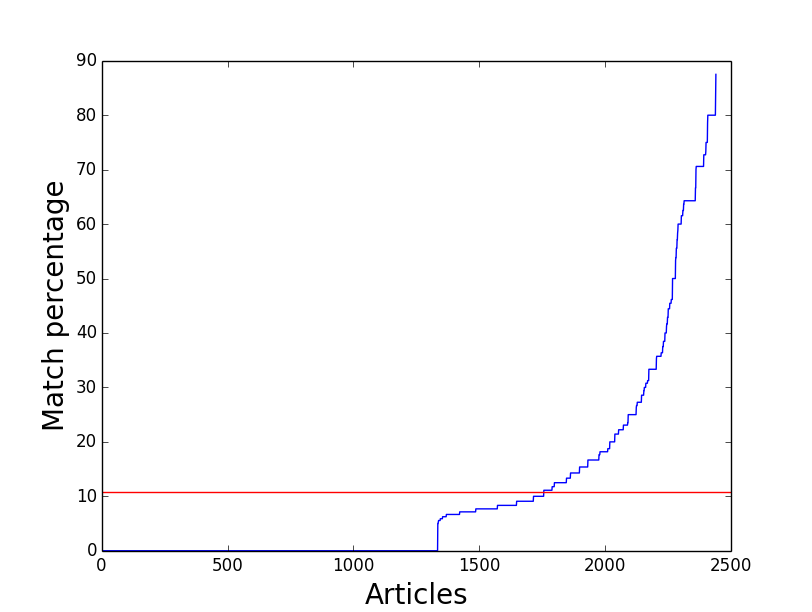
\includegraphics[width=0.7\textwidth, height=9cm]{bigrammatch}
\caption[Bigram match percentages]{Distribution of bigram match percentage over the tweet-article pair. The mean here is 10.73\% shown by the red horizontal line, with a standard deviation of 18.5\%}
\label{fig:bigrammatch}
\end{figure}


\section{Percentage Match for Bigrams}
\label{sec:bigrams}

Similar to the unigram matching techniques, the bigram percentage matching was also calculated. The text of the tweet was converted into bigrams and we then looked for those bigrams in the article text. The percentage was calculated similar to the unigram matching done earlier. For the set of bigrams for a text $x$, $\textit{bigrams}(x)$, percentage of matching bigrams $b$ for the tweet $t$ and article $a$ is: 

\begin{equation}
b = \frac{| \textit{bigrams}(t) \cap \textit{bigrams}(a) |}{| \textit{bigrams}(t) |} * 100
\end{equation}

\figref{fig:bigrammatch} shows the percentages of matched bigrams found. The mean is 10.73 with a standard deviation of 18.5. As seen in the figure, most of the tweet-article pairs have no matched bigrams. The percentage then increases to reflect the complete matches found above.

\begin{figure}[!htbp]
\centering
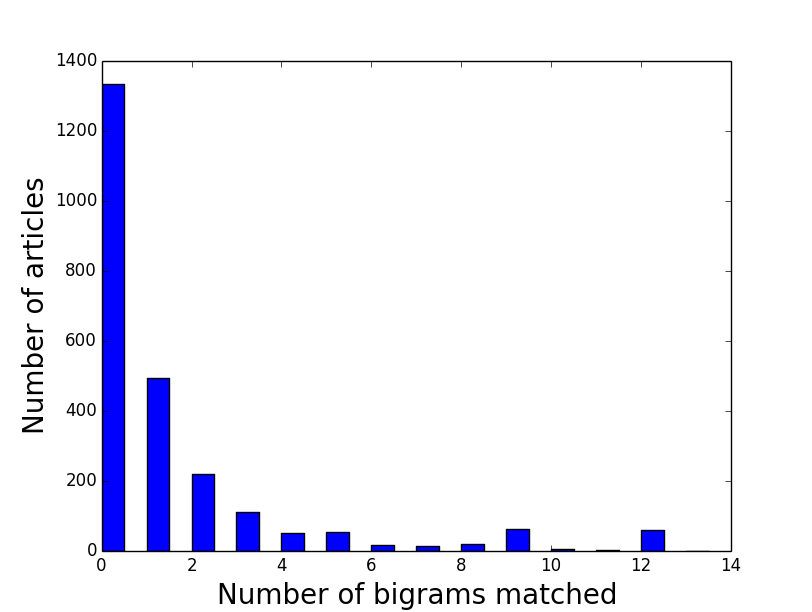
\includegraphics[width=0.7\textwidth, height=9cm]{num_bigrams}
\caption[Histogram for number of matched bigrams.]{Histogram of number of unique tweet-article pairs vs number of bigrams matched. The mean number of bigrams matched per article is 1.9.}
\label{fig:num_bigrams}
\end{figure}

\figref{fig:num_bigrams} shows frequency of the number of tweet-article pairs for the number of bigrams matched. There are no matched bigrams for most of the pairs. A smaller number of articles had one matched bigram, and the number decreased until the end, where it increases a little at more than 10 matched bigrams because of exact tweet matches. 


\section{Percentage Match Inside a Window in the Article Text}
\label{sec:window}

The next analysis checks for a significant word matching inside a three-sentence window inside the article text. We used a three sentence long window using the sentence boundary information obtained during preprocessing. A window of three sentences was chosen to give a smaller context for the tweet to be extracted from than the entire article. The number was chosen as a moderate context window size as not too small to reduce it to a sentence level, and not too big for the context to be diluted. This was done to investigate whether a pseudo-extractive multi-sentence compression approach could convert a small number of sentences into a tweet.

After the text of the window was extracted, we performed a similar analysis as the last one, except on a smaller set of sentences. The matching percentages from all three-sentence windows in the articles were computed and the maximum out of these was taken for the final results. Let a sentence window $w_i$ be the set of three consecutive sentences starting from the sentence number $i$. For this window, the unigram match in the tweet $t$, and the window is the unigram match $u$ calculated above. Then, the maximum match from all the windows, $uw$ is 

\begin{equation}
uw = max_{w_i \in S} u(t, w_i)
\end{equation}

\begin{figure}[!htbp]
\centering
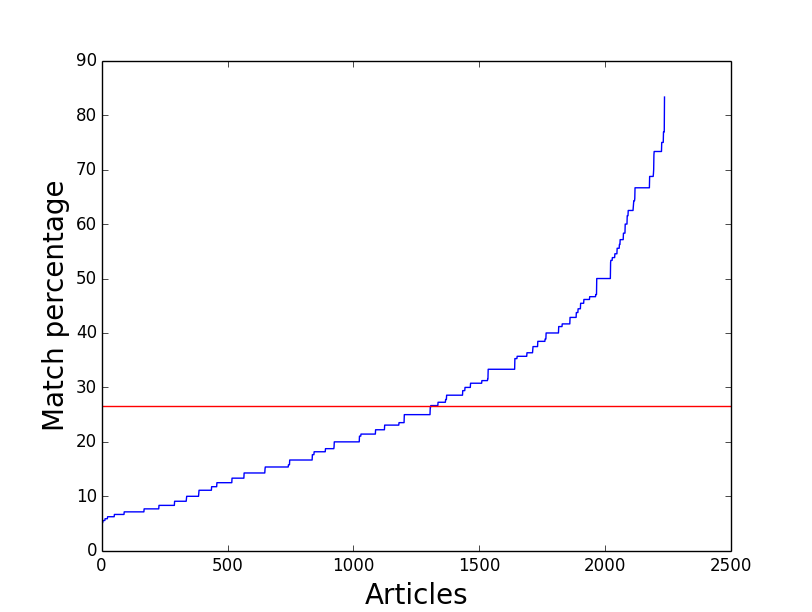
\includegraphics[width=0.7\textwidth, height=9cm]{unigramwindow}
\caption[Match percentages in tweet against window in article]{Percentages of common words in tweet and a three sentence window in the article. The maximum match from all percentages is chosen for an article. The red horizontal line is the mean is 26.6\%, and standard deviation 17\%.}
\label{fig:unigramwindow}
\end{figure}

The result from this experiment is shown in \figref{fig:unigramwindow}. Here, the mean of the values is 26.6\% and deviation 17\%. Again this shows that only a small proportion of tweets can be generated even with an approach that combines unigrams from multiple sentences in the article.


\section{Longest Common Subsequence Match Inside a Window for the Text}
\label{sec:lcs}

\begin{figure}[!htbp]
\centering
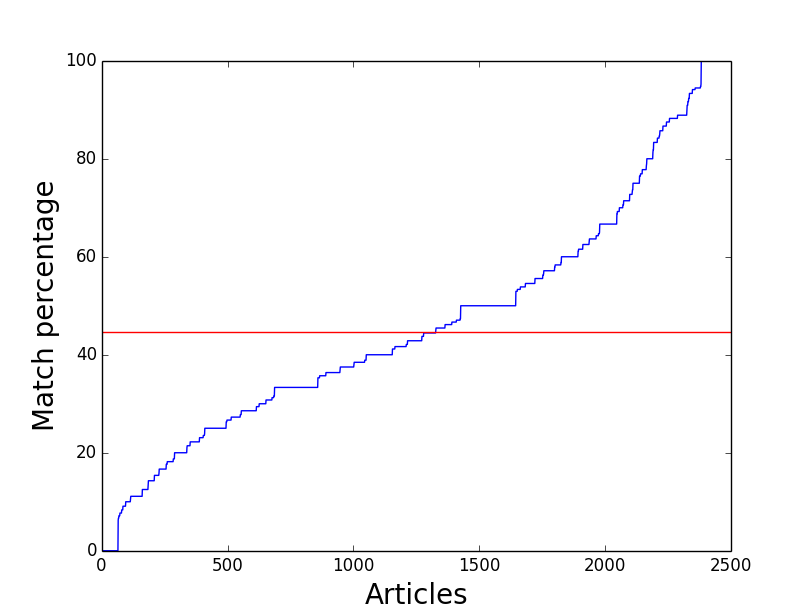
\includegraphics[width=0.7\textwidth, height=9cm]{lcs_doc}
\caption[match]{Percentages of words matching in tweet and document text using an LCS algorithm. Mean is 44.6\%, which is shown by the red horizontal line, and standard deviation is 22.7\%.}
\label{fig:lcs}
\end{figure}

The percentage match analyses were a bag-of-words approach that disregarded the order of the words inside the texts and tweets. To respect the order of the words in the sentence of the tweet, we also used the least common subsequence algorithm between the tweet text and the document text. This subsequence matching was done inside a sentence window of 5 sentences. 
Again, the final result for the article was the window in which the maximum percentage was recorded among all windows. The percentage match was calculated using the number of words in the tweet as the denominator.

If $\textit{lcs(t, a)}$ is the longest common subsequence between the tweet $t$ and article $a$, $\textit{unigrams}(x)$ is the set of unigrams for a text $x$, then the percentage of match for the lcs as compared to the tweet, $\textit{l}$ is


\begin{equation}
l = \frac{| \textit{lcs}(t, a) |}{| \textit{unigrams}(t) |} * 100
\end{equation}


 These numbers are shown in \figref{fig:lcs}. The mean here is 44.6\% and the standard deviation is 22.7\%. 

\section{Interaction with Formality}

As seen in the results of the analyses performed in \chapref{chap:analysis}, the tweets have little in common with the articles they are linked to. This shows that extractive summarization algorithms can only recover a small proportion of the indicative tweets. To tie in the results of the findings above with some intuitive notions about the text and see how formality interacts with the results, we also calculated the formality of the articles. This formality score was correlated with the longest common subsequence measure that we defined above. 

We assume that the formality of an article can be estimated by the formality of the words and phrases in the article. We used the formality lexicon of \cite{brooke2013multi}. They calculate formality scores for words and sentences by training a model on a large corpus based on the appearance of words in specific documents. Their model represents words as vectors and the formal and informal seeds appear in opposite halves of the graphs, suggesting that we can use these seeds to determine if an article is formal or informal. The lexicon consists of words and phrases and their degree of formality. Thus, more formal words are marked on a positive scale and informal words like those occurring in colloquial language are marked on a negative scale. 

Let the set of formality expressions from the lexicon be $L$, and the formality score for an expression $e$ be $\textit{score}(e)$. Let the set of all substrings from the article $\textit{substrings}(a)$ be $S$. Then, the formality score $f$ for an article $a$ is the number of formal expressions per 10 words in article is   

\begin{equation}
f = \frac{\sum\limits_{e \in L \& e \in S} \textit{score}(e)}{| \textit{unigrams}(a) |} * 10
\end{equation}

The formality lexicon gave positive weights for formal expressions and negative for informal expressions. When we computed $f$ using both formal and informal expressions, we found that the informal words predominated and ``swamped'' the signal of the formal words, leading to incomprehensible results. Thus, we discarded the informal words and used only the weights from the formal words in our final calculations. To check that these formality scores made sense intuitively, we calculated the average formality score for the articles belonging to each hashtag and ordered them, as shown in \tabref{tab:formal}.

\begin{table}[!htbp]
\centering
\begin{tabular}{|l|l|}
\hline
Lowest  & Highest  \\ \hline
\#theforceawakens       & \#KevinVickers           \\
\#TaylorSwift           & \#erdogan                \\
\#winteriscoming        & \#apec                  \\ \hline
\end{tabular}
\caption[Order of formality ranking in hashtags]{Table of hashtags (broadly, topics) with highest and lowest formality according to the lexicon.}
\label{tab:formal}
\end{table}


\begin{table}[!htbp]
\centering
\begin{tabular}{|p{0.1\linewidth}|p{0.8\linewidth}|}
\hline
Tweet &  @globetoronto: Why Buffalo got clobbered with snow and Toronto did not. \#weather \#snowstorm http://t.co/gcwwoDPZmX... http://t.co/BXY7EH6F3u" \\ \hline
Title & What caused Buffalo’s massive snow and why Toronto got lucky \\  \hline
Text  & Torontonians have long been the butt of jokes about calling in the army every time a few snow flurries whip by... \\ \hline
\end{tabular}
\caption[Example of formality in article affecting tweet]{Example of a tweet, title of the article where the formality of the article is over the mean, and the tweet is extracted from the article.}
\label{tab:formalexample}
\end{table}

This formality score for each article was correlated with the percentage of match obtained using the longest common subsequence algorithm. The Pearson correlation value was 0.41, with a p-value of 7.08e-66, indicating that the interaction between formality and overlap was highly significant. Hence, we can say that the more formal the subject or the article, the better the tweet can be extracted from the article. \tabref{tab:formalexample} gives an example of the formality of the article, which is a low 4.2 formality words per 10 words, where the tweet is not extracted from the article, but rephrased from the article instead.

We speculate that tweets associated with less formal articles may contain more abbreviations and non-standard words or spellings, which decreases the amount of overlap. To counter this case, we tried experimenting with word normalization systems which could resolve words like '2mw' or '4eva' to 'tomorrow' and 'forever' respectively. Systems described by \cite{yang2013log} and \cite{gouws2011contextual} were tested with our data. Unfortunately, neither provided the results we suitable enough to integrate with our analyses, and this will be something to look into further upon development of more accurate word normalization systems. 




\chapter{User Study}
\label{chap:user}

% More details on the paper.
\chapref{chap:analysis} describes the analyses performed on the data and the resulting conclusion, that only a small portion of indicative tweets can be recovered from the article they link to if viewed as an extractive summarization problem. This conclusion suggests that the next step should be gaining more knowledge about the relation between the tweet and the article in terms of what the tweet does with respect to the article. This information would enable us to figure out if a tweet can actually be generated from summarizing the text in the article. If so, we would then be able to figure out what strategy would be the most appropriate for this task. This task has been explored in this chapter. 

\section{Functions of Tweets}
% Preliminary recommendations on text typology
One aspect of gaining more knowledge would be asking what the \textit{`function'} of the tweet is. If the function of the tweet is known, it might be possible to predict the degree of extractiveness of the tweet with respect to the article. For example, if the function of the tweet is to be an advertisement for a particular product and the text contains the description of the features of the product, then intuitively, the tweet would likely be an extractive summary of the text. On the other hand, if the tweet were an attention grabbing title to merely bring traffic to the text, it would be more likely to be a generic title, than a summary of the actual text. To identify these functions, we first looked at multiple studies aiming to classify functions of tweets. Once functions were isolated and questions to be asked about the tweets finalized, the data was put forth to be classified by human evaluators in a user study.

\subsection{Previous work in classifying function of tweets}
%Having learnt from the tagging attempts earlier, we think that one promising direction is to model the \textit{function}, more explicitly. 
There have been several studies on classifying function of tweets, but in many cases it is described as a more general, high-level intents of the tweets, akin to classifying the topic or genre of the tweet rather than the function. \cite{wang2015mining} use bootstrapping to generate an intent keywords set used in generating an intent graph in a semisupervised manner. They focus on finding tweets with intent and then classifying those. The intent here is defined as a wish or a plan to for some action, such as intent for buying/doing food and drink, travel, career and so on. Classification of intents in this way can directly be used as intents for purchasing and be utilized for advertisements.  \citet{banerjee2012towards} analyze real time data to detect presence of intents in tweets. \citet{gomez2014content} use features from text and stylistics to determine user intentions, which are classified as news report, opinion, publicity and so on. \cite{mohammad2013identifying} use a different take on the intents and use them to study the classification of user intents specifically for tweets related to elections. They study one election and classify tweets as ones that agree or disagree with the candidate, ones that are meant for humour, support and so on. 
%These definitions of intent, while a promising start, will not be sufficient for tweet generation. For this purpose, intent would be the reason the user chose to share the article with that particular text. \cite{sinclair1996preliminary} describe this as 'communicative intent' describing the types as information, discussion, recommendation, recreation, religion and instruction with further subcategories. 


\subsection{Possible functions and questions}

While the definitions described earlier are a promising start, we were looking for a way to model the function in the sense of why the user chose to share the article with the particular text written in the tweet. The closest description found was in \cite{sinclair1996preliminary}, who describe this as `communicative intent' describing the types as information, discussion, recommendation, recreation, religion and instruction with further subcategories. There are also the traditional summary classifications such as evaluative vs descriptive and informative, indicative and critical. 

The first attempt at tagging the dataset were made using the following scheme: a sample set of 100 articles were tagged by two people. The tags used in the preliminary tagging were : `evaluative' vs `descriptive'. `Evaluative' text is a more opinionated text, that is more subjective. This text would be expected to take a certain object or event, analyze it,  and form an opinion about it. `Descriptive' text is non-evaluative, containing for example a narration of an event or an explanation about a certain object or event. A `mixed' category was also added to accommodate some in-between articles. The tagging was done based on the title, article text and tweet. It was observed that this classification was rather subjective, especially between the evaluative/descriptive/mixed tags. Consequently, the Cohen's kappa \citep{kohen1960coefficient} value for correlation turned out to be 0.13, confirming the difficulty of distinguishing these tags. \cite{liu2012survey} give a detailed analysis about classifying evaluative vs descriptive texts, the task is named as subjectivity classification. They point out that it is a bad idea to classify on a sentence level in complex sentences, since a sentence and by extension a text might be factual as well as evaluative, which was the original problem while tagging. These tagging schemes did not yield much success in terms of gleaning information over the entire dataset.

The type of articles being referenced, and the possible reasons these might be shared gave the list of the possible functions. Using these and earlier studies, we enumerated the relevant functions of tweets for our data : promote a product or an article, agree or disagree with an event, or express an opinion about it. Identifying these functions would ideally help provide parameters for generating tweets. These idea behind these functions have been discussed in the following paragraphs. 

If the tweet references a newspaper article, it might be promoting the article, in the sense of attracting people to go further and read the article in more detail. This kind of tweet would try to sensationalize material. It could either tweet the headline of the article directly, or summarize the headline itself further, or simply says something in the likes of `Check this out' or `This is worth a read' and then further categorizes the article with the use of appropriate hashtags indicating the contents of the text.

Example :``Check out this article! \{url\}" or ``Look what this says! \{url\}"

A second option is that the tweet expresses an opinion about something in the article. It could be a positive or a negative comment about the contents of the article or an agreement or disagreement about the events or thoughts and opinions expressed in the article. 

Example : "This is a terrible analysis. {url}" or "Listening to this album on repeat! {url}"

And thirdly, it could be a tweet that singles out a particular piece of information or opinion directly from the article, either to agree with it or to express the importance of the sentence or phrase in the article according to the author of the tweet. It could also be a short summary of the text of the article to either with the aim of inviting readers or just inform readers about the contents of the article.

Example :``Winter approaching, ways to stay safe from flu season: \{url\}"


\section{Running User Study on Amazon Mechanical Turk}

Amazon Mechanical Turk is a crowdsourcing platform that enables researchers to put up huge samples of data along with surveys, quizzes, and simple tasks to be solved by people over the world.

\subsection{Pilot Studies}

 Four pilot studies were conducted on 100 randomly selected tweet and article pairs, using each to improve the questions. For these pilot studies, we tried various combinations of questions and qualifications.
 
 \paragraph{Questions used} All the questions described earlier were experimented with, with the question about emotion giving the highest Fleiss' kappa \citep{geertzen2012inter} between the raters. Since this question was included as a point of interest for future studies, it was dropped going forward with the rest of the studies.
%  The questions used in these studies were the two described above along with another question asking whether the tweet expressed an emotion about the article. It could be a positive or a negative comment about the contents of the article or an agreement or disagreement about the events or thoughts and opinions expressed in the article. 
 
%  Example :``This is a terrible analysis. \{url\}" or ``Listening to this album on repeat! \{url\}"


\paragraph{Qualification settings} Mechanical Turk assigns qualifications to workers based on their skill level in answering questions and their statistics in accepted answers. Workers with superior skills and higher accuracy while answering HITs get the qualification `Masters' which was the qualification used for these pilot studies.

Three separate opinions from the workers were gathered for each tweet and article pair and the agreement calculated using Fleiss' kappa measure  of agreement \citep{geertzen2012inter} between the raters. These pilot studies paved the way towards understanding how the data was being analyzed by outsiders. 
 
 
  % A second option is that the tweet expresses an opinion about something in the article. It could be a positive or a negative comment about the contents of the article or an agreement or disagreement about the events or thoughts and opinions expressed in the article. 

% Example : "This is a terrible analysis. {url}" or "Listening to this album on repeat! {url}"

\subsection{Questions used for the final study}

After the four initial pilot studies, a decision was taken to present the questions separately in two different studies excluding the third question about emotion expressed by tweet. This would guarantee an unbiased opinion about that particular question without any assumptions of either/or questions.

The final questions derived from these functions are shown in \tabref{tab:mturkqs}. A third question of whether the tweet expressed an emotion towards the article, and if so, whether it was a positive or negative emotion was asked too for the purpose of data collection. 

\begin{table}[!htbp]
\centering
\begin{tabular}{|p{0.15\linewidth}|p{0.8\linewidth}|}
\hline
Question 1 & Does the tweet explicitly encourage the reader to visit the link and read the original article? \\ \hline
Question 2 & Does the tweet contain some information from the article, or summarize the article?             \\ \hline
\end{tabular}
\caption{Questions for user study}
\label{tab:mturkqs}
\end{table} 

\subsection{Qualification details}

After playing with the initial setting of `Masters' on the Mechanical Turk, we found the way to obtain the best quality results was to add an additional level of qualification. The qualification test contained three questions from the dataset that had an obvious category for function of tweets. These tests were presented to the workers, and only workers with a 100\% score in these tests were allowed to work on the data. These tests would ensure not only that the worker had a complete understanding of the task at hand, but also be able to come to a correct conclusion in an obvious category situation. A separate pilot with these qualifications and questions structure gave promising results, and the user study was then run on the entire dataset.

\subsection{Running the final study}

\figref{fig:q1} and \figref{fig:q2} show an example of what a HIT (task on Mechanical Turk) for the two questions looked like to the user, respectively.
\begin{figure}[!htbp]
  \centering 
  \subfloat{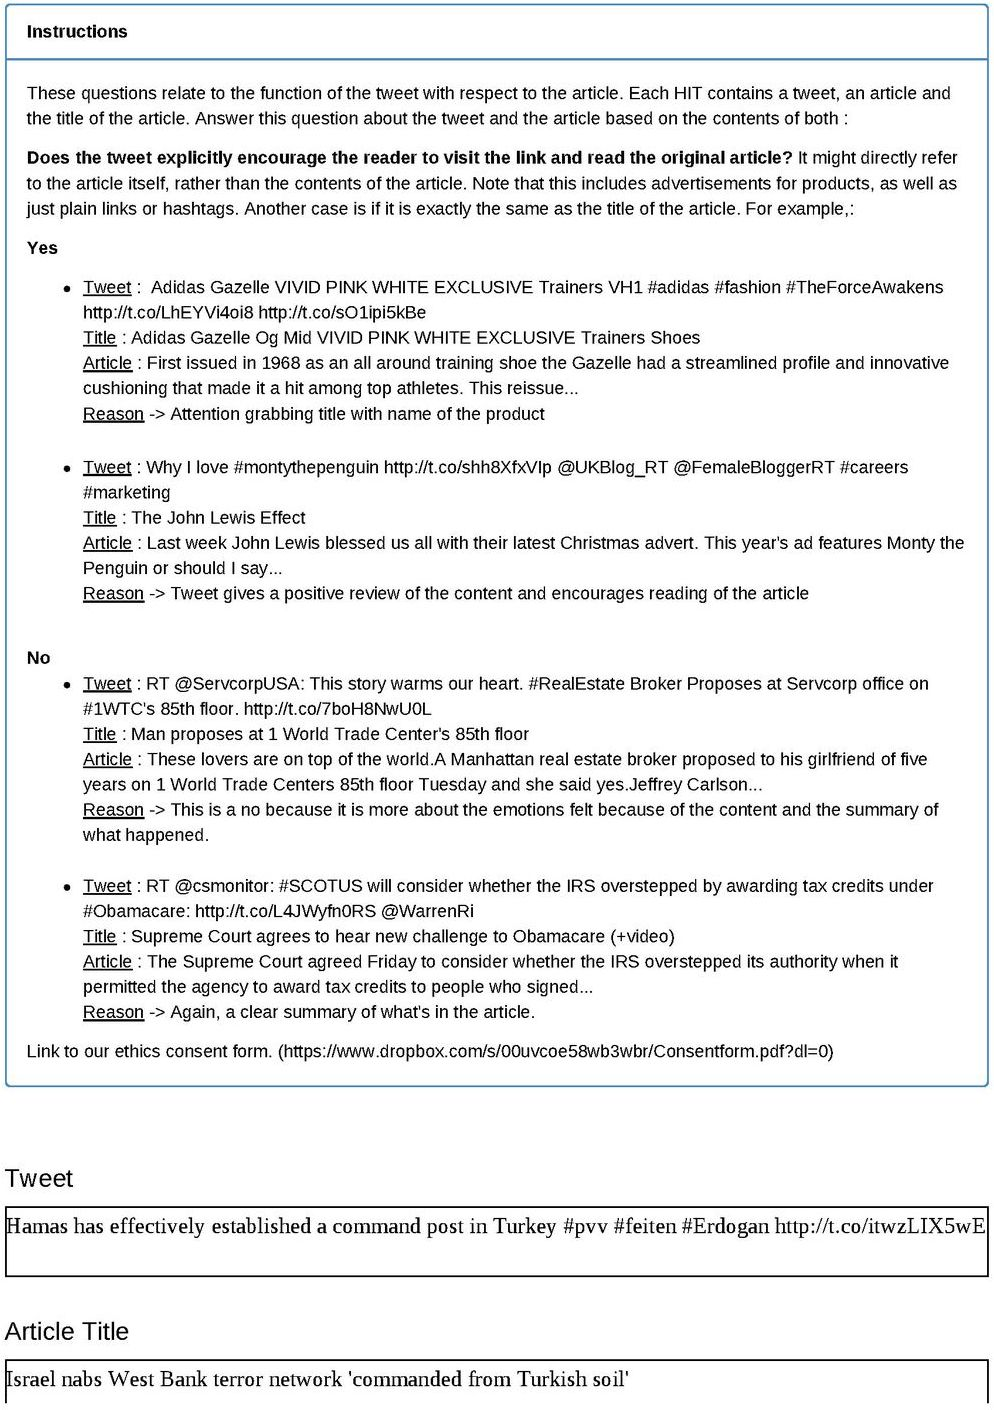
\includegraphics[width=\textwidth, height=21cm]{q11}}
  %\qquad 
  %\subfloat[][b]{q11} 
  \caption[User study question 1 example]{The first question posed for each sample asked to the users.}
  \label{fig:q1}
\end{figure}

\begin{figure}[!htbp]
  \ContinuedFloat 
  \centering 
  \subfloat{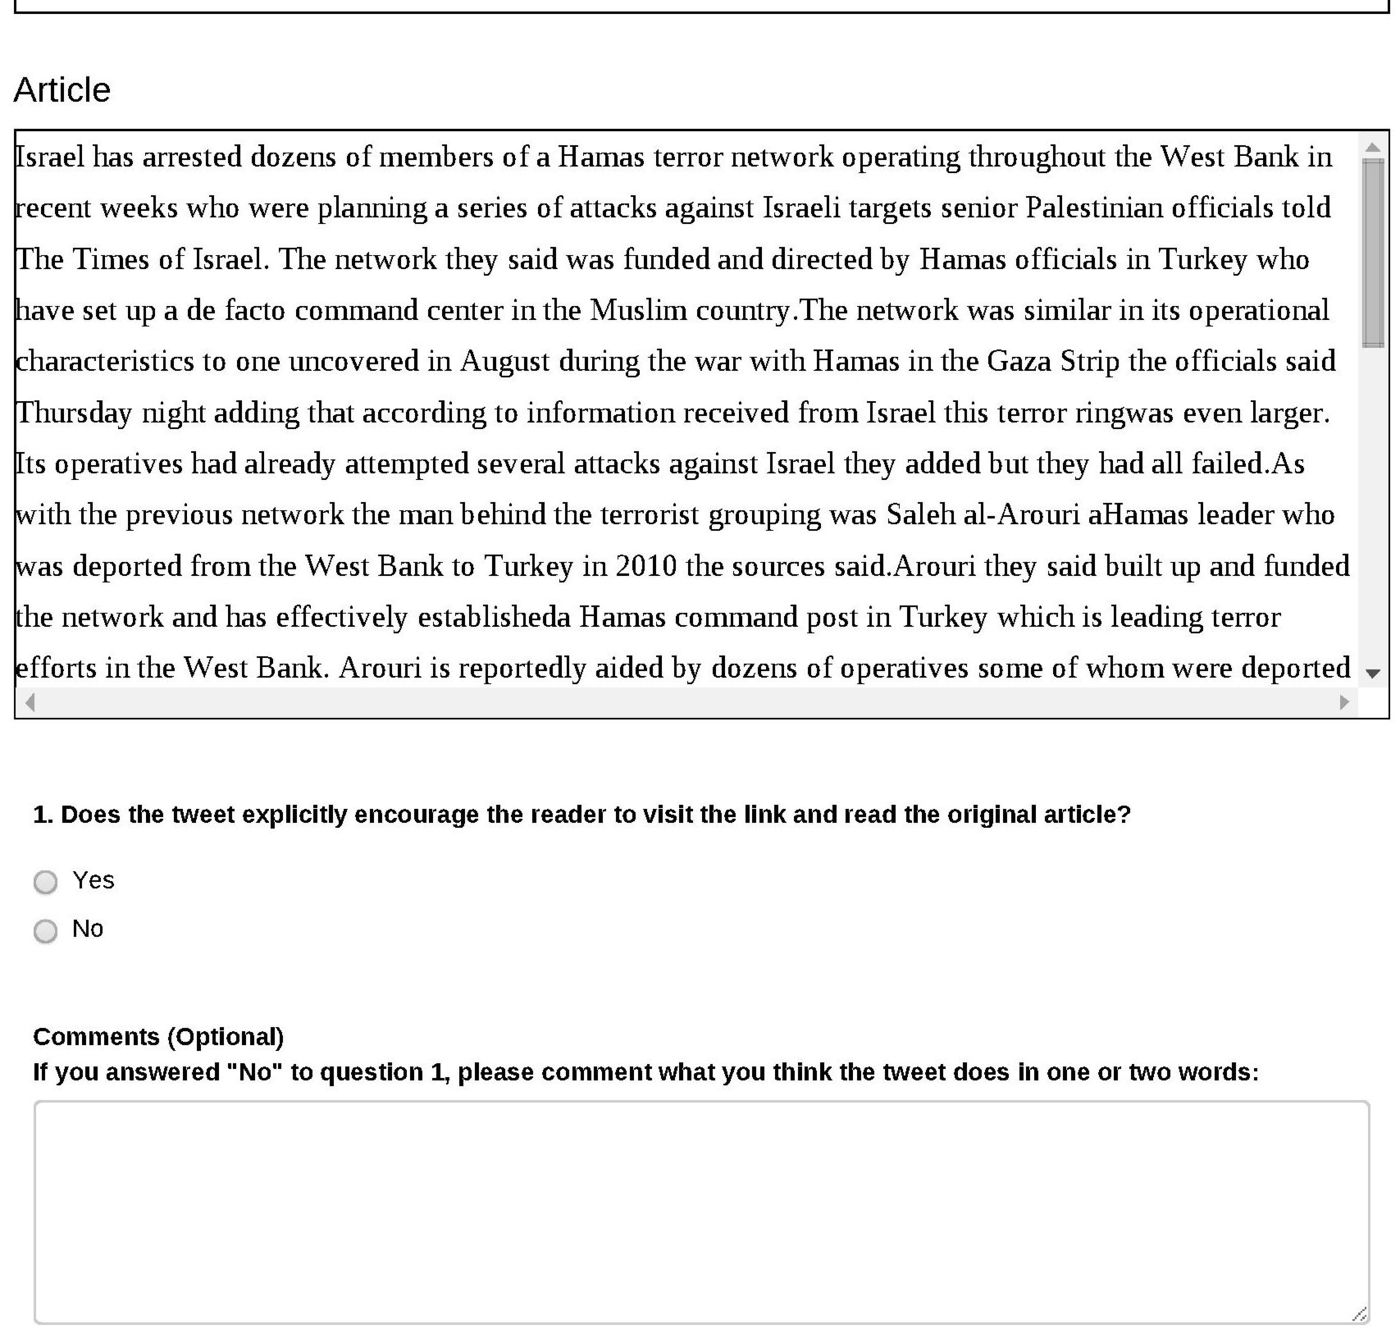
\includegraphics[width=\textwidth, height=13cm]{q12}}% 
  %\qquad 
  %\subfloat[][]{q12} 
  \caption[]{..continued question viewed by users.}
  \label{fig:q12}
\end{figure} 

\begin{figure}[!htbp]
  \centering 
  \subfloat{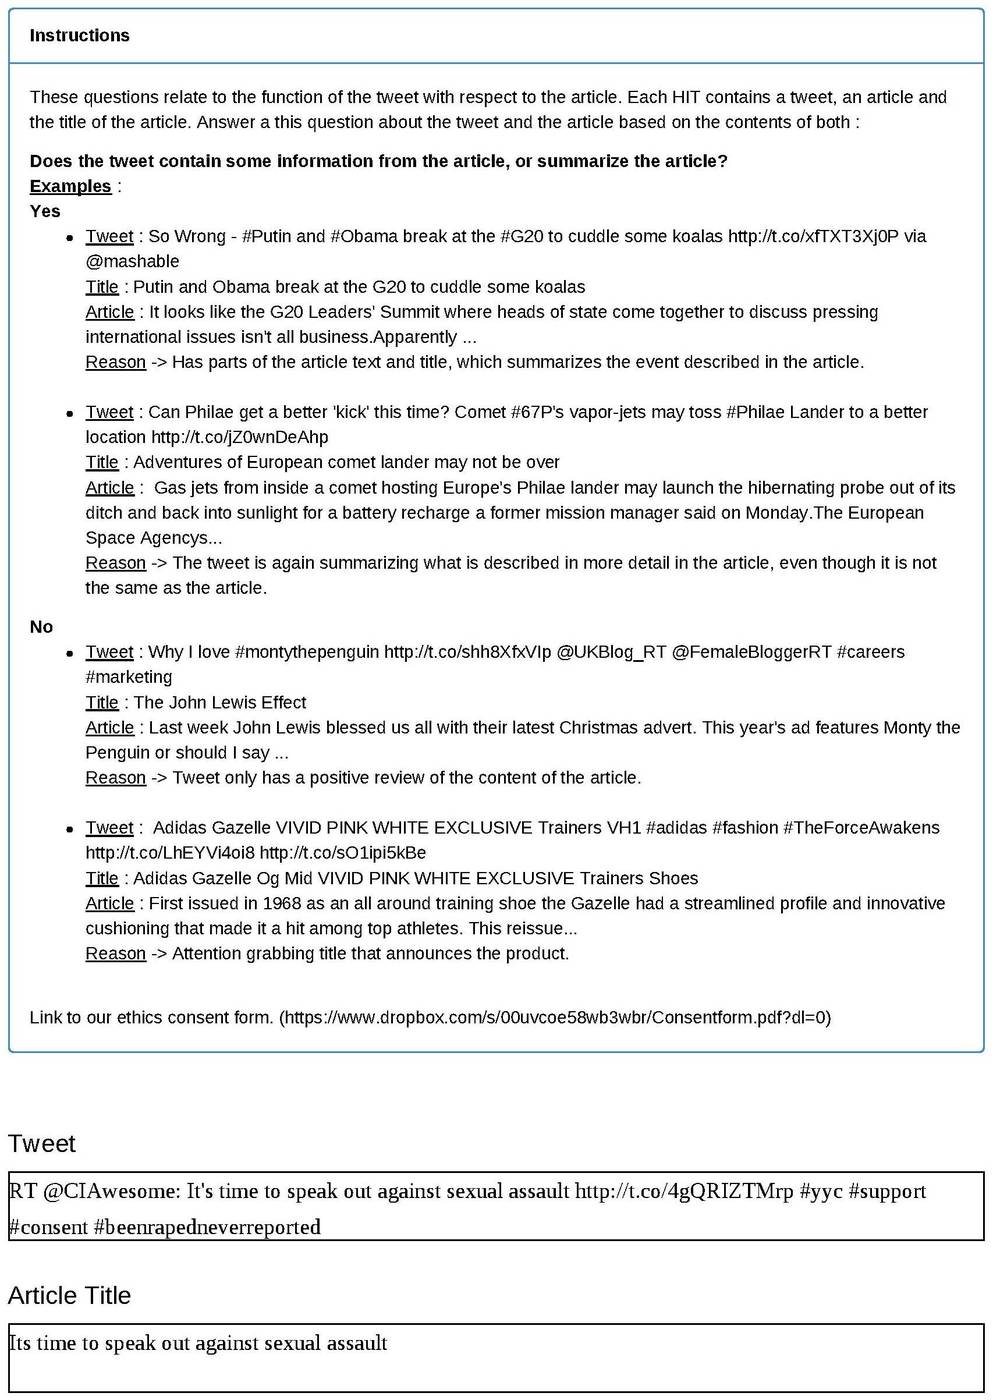
\includegraphics[width=\textwidth, height=21cm]{q21}}
  %\qquad 
  %\subfloat[][b]{q11} 
  \caption[User study question 2 example]{The second question asked for each sample.}
  \label{fig:q2}
\end{figure}

\begin{figure}[!htbp]
  \ContinuedFloat 
  \centering 
  \subfloat{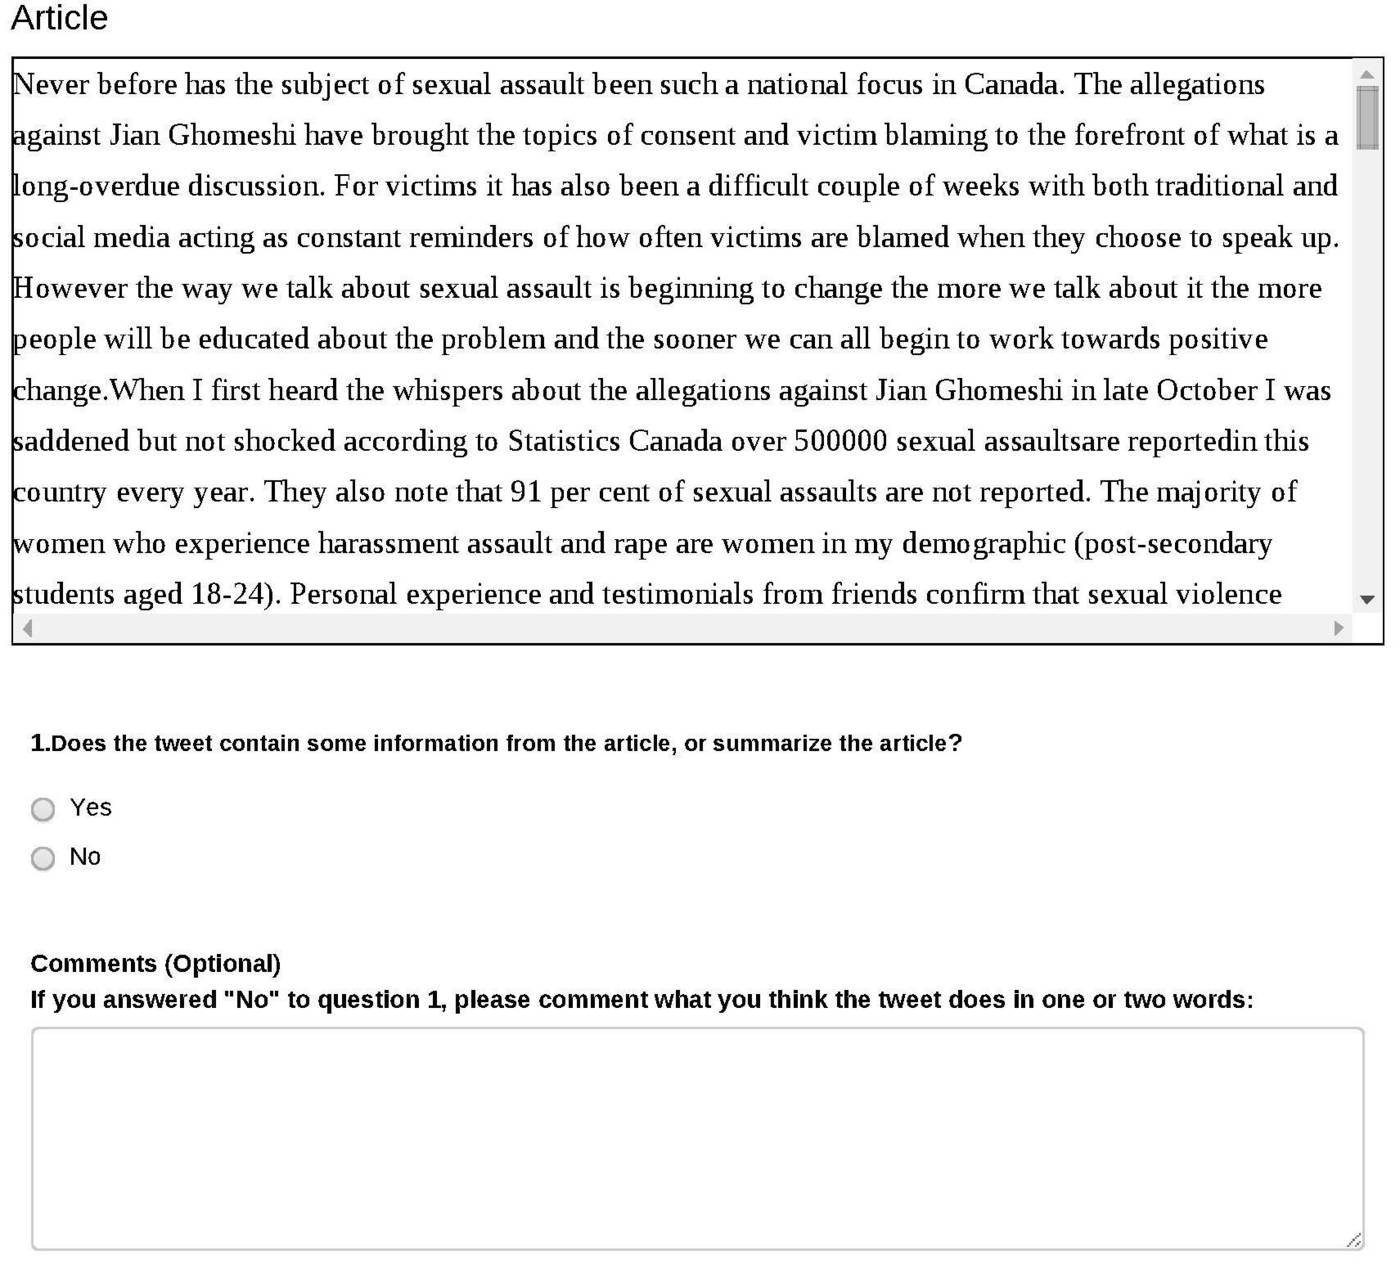
\includegraphics[width=\textwidth, height=13cm]{q22}}% 
  %\qquad 
  %\subfloat[][]{q12} 
  \caption[]{..continued question viewed by users.}
  \label{fig:q22}
\end{figure} 

% * analysis of results from MTurk
%finally separated user studies, 4 pilots
%qualification tests
%mechanical turk CLI
%add forms 
% results can be added later

\subsection{Results and Analysis for User Study}

% \begin{figure}[!htbp]
% \centering
% 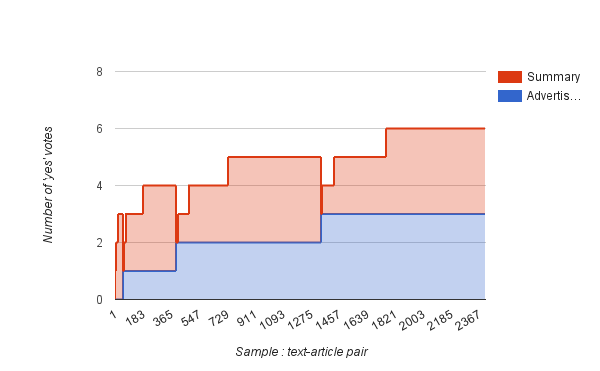
\includegraphics[width=0.9\textwidth, height=9cm]{results}
% \caption[Results from user study]{Visualization for tags from human evaluators}
% \label{fig:res}
% \end{figure}

% The results obtained from the final study are shown in \figref{fig:res}. The bottom line shows the number of 'yes' votes per article and tweet for the first question, whether the tweet was a promotion of the article. The red line on top of it signifies the number of 'yes' votes for the second question, whether the tweet was a summary of the article. 

The total number of `yes' votes for each of the questions are shown in \tabref{tab:yeses}. \tabref{tab:exq1no}, \tabref{tab:exq1yes}, \tabref{tab:exq2no} and \tabref{tab:exq2yes} all show examples where for one of each question, all three workers agreed to a tweet being or not being an advertisement or a summary. The Fleiss' kappa for the first study, showing the indicativeness of the tweet was 0.147 and the kappa for the second study, showing the informativeness of the tweet, was 0.208.

\begin{table}[!htbp]
\centering
\caption{Analysis of user study results}
\label{tab:yeses}
\begin{tabular}{|l|l|l|l|l|}
\hline
Questions     & 0 votes & 1 vote & 2 votes & 3 votes \\ \hline
Advertisement & 53    & 340    & 942     &  1068  \\ \hline
Summary       & 29     & 176    & 703     & 1495    \\ \hline
\end{tabular}
\end{table}


\begin{table}[!htbp]
\centering
\begin{tabular}{|p{0.1\linewidth}|p{0.8\linewidth}|}
\hline
Tweet &   RT @WSJ: In \#CometLanding Philae probe bounced and settled in area that could hinder its research. http://t.co/6lfg3p9XG1 http://t.co/A6fi  \\ \hline
Title &   Rosetta Mission Probe Landed on Comet in Shadow of Cliff	                                                                                 \\ \hline
Text  &  The historic Philae comet probe hit its target but then unexpectedly bounced twice settling in the shadow of a cliff that could hinder its research new images sent back Thursday showed.Philae is designed to run a suite...                                                                                         \\ \hline
\end{tabular}
\captionof{table}{Example where all three workers said it was not an advertisement.}
\label{tab:exq1no}
\end{table}


\begin{table}[!htbp]
\centering
\begin{tabular}{|p{0.1\linewidth}|p{0.8\linewidth}|}
\hline
Tweet & \#GalaxyNote3 \#Lollipop - SamMobile has been teasing us with a number of unfinished builds for a few http://t.co/A0IKYsk4g3 \#Samsung \\ \hline
Title &   Samsung GALAXY Note 3's Android Lollipop Update Surfaces                                                                                 \\ \hline
Text  &  SamMobile has been teasing us with a number of unfinished builds for a few months now. This indicates...                                                                                         \\ \hline
\end{tabular}
\captionof{table}{Example where all three workers said the tweet was an advertisement for article.}
\label{tab:exq1yes}
\end{table}


\begin{table}[!htbp]
\centering
\begin{tabular}{|p{0.1\linewidth}|p{0.8\linewidth}|}
\hline
Tweet & "RT @jakbarali: So my partner Gillian Hnatiw and I had something to say about \#VAW \#LoriDouglas and \#Ghomeshi. http://t.co/6X2zMtCAM0 \\ \hline
Title & "Victim-blaming couched as legitimate judicial inquiry" \\ \hline
Text  & Ghomeshi himself broke the first wave of the story when he took to Facebook to decry the CBCs decision to terminate him... \\ \hline
\end{tabular}
\captionof{table}{Example where all three raters said tweet was not a summary.}
\label{tab:exq2no}
\end{table}

\begin{table}[!htbp]
\centering
\begin{tabular}{|p{0.1\linewidth}|p{0.8\linewidth}|}
\hline
Tweet & RT @PopCulturPriest: Doing a story on California's lottery for @americmag I discovered \#JohnOliver's story had some troubling errors: http \\ \hline
Title & Blowing The Dismount: Last Week Tonight Fudges Its Lottery Story \\ \hline
Text  & Sunday night on the season finale of HBOs new news show Last Week Tonight anchor John Oliver spent half the show... \\ \hline
\end{tabular}
\captionof{table}{Example where all three raters agreed the tweet was a summary.}
\label{tab:exq2yes}
\end{table}

We then analyzed the tags obtained from the study with the analyses results we obtained in \chapref{chap:analysis}. The results for the Mann Whitney U test \citep{mann1947test,wilcoxon1947probability} with different parameters considered are shown. \tabref{tab:unicorr1} and \tabref{tab:unicorr2} show the test results for unigram match percentages, \tabref{tab:bicorr1} and \tabref{tab:bicorr2} for bigram match percentages, and \tabref{tab:lcscorr1} and \tabref{tab:lcscorr2} for longest common subsequence match percentages. Each of these are for the two separate studies respectively.  The test was first done while considering zero `yes' votes as one group and three `yes' votes as another group. The test was also done considering zero or  one `yes' votes out of three in one group and two or three `yes' votes out of three in the other group. For each of these studies for each sample set configuration, the U statistic and the p value are shown. The final two columns in both tables show the mean values of values in each of the groups used in the test. 
%The failure to reject the null hypothesis suggests that no definite distinction can be made between the degree of extraction for tweets that are advertisements for articles or summaries of articles.

\begin{table}[!htbp]
\caption{Mann Whitney U test results for indicativeness: Unigram Match}
\centering
\label{tab:unicorr1}
\begin{tabular}{|p{0.29\textwidth}|p{0.1\textwidth}|p{0.1\textwidth}|p{0.09\textwidth}|p{0.09\textwidth}|p{0.09\textwidth}|p{0.09\textwidth}|}
\hline
Groups considered    & U statistic & p value & Mean of values for Group 1 & Number of samples in Group 1 & Mean of values for Group 2 & Number of samples in Group 2\\ \hline
Group 1: 0 `yes' votes \newline Group 2: 3 `yes' votes &  28104  &  0.931413  &  27.44  & 53 & 28.21 &   1068  \\ \hline
Group 1: 0 or 1 `yes' votes \newline Group 2: 2 or 3 `yes' votes &   406355.5  & 0.365219 & 30.65  & 393 & 29.23 & 2010 \\ \hline
\end{tabular}
\end{table}

\begin{table}[!htbp]
\caption{Mann Whitney U test results for informativeness: Unigram Match}
\centering
\label{tab:unicorr2}
\begin{tabular}{|p{0.29\textwidth}|p{0.1\textwidth}|p{0.1\textwidth}|p{0.09\textwidth}|p{0.09\textwidth}|p{0.09\textwidth}|p{0.09\textwidth}|}
\hline
Groups considered    & U statistic & p value & Mean of values for Group 1 & Number of samples in Group 1 & Mean of values for Group 2 & Number of samples in Group 2\\ \hline
Group 1: 0 `yes' votes \newline Group 2: 3 `yes' votes & 12211 & 0.000055  & 16.69 & 29 & 31.07 & 1495  \\ \hline
Group 1: 0 or 1 `yes' votes \newline Group 2: 2 or 3 `yes' votes & 193411 & 0.000791 & 25.08 & 205 & 29.87 & 2198 \\ \hline
\end{tabular}
\end{table}

\begin{table}[!htbp]
\caption{Mann Whitney U test results for indicativeness: Bigram Match}
\centering
\label{tab:bicorr1}
\begin{tabular}{|p{0.29\textwidth}|p{0.1\textwidth}|p{0.1\textwidth}|p{0.09\textwidth}|p{0.09\textwidth}|p{0.09\textwidth}|p{0.09\textwidth}|}
\hline
Groups considered    & U statistic & p value & Mean of values for Group 1 & Number of samples in Group 1 & Mean of values for Group 2 & Number of samples in Group 2\\ \hline
Group 1: 0 `yes' votes \newline Group 2: 3 `yes' votes & 27871 & 0.851388 & 8.31 & 53 & 9.21 & 1068  \\ \hline
Group 1: 0 or 1 `yes' votes \newline Group 2: 2 or 3 `yes' votes& 406313 & 0.378553 & 12.19 & 393 & 10.29 & 2009 \\ \hline
\end{tabular}
\end{table}

\begin{table}[!htbp]
\caption{Mann Whitney U test results for informativeness: Bigram Match}
\centering
\label{tab:bicorr2}
\begin{tabular}{|p{0.29\textwidth}|p{0.1\textwidth}|p{0.1\textwidth}|p{0.09\textwidth}|p{0.09\textwidth}|p{0.09\textwidth}|p{0.09\textwidth}|}
\hline
Groups considered    & U statistic & p value & Mean of values for Group 1 & Number of samples in Group 1 & Mean of values for Group 2 & Number of samples in Group 2\\ \hline
Group 1: 0 `yes' votes \newline Group 2: 3 `yes' votes & 15006 & 0.004541 & 3.88 & 29 & 11.46 & 1494  \\ \hline
Group 1: 0 or 1 `yes' votes \newline Group 2: 2 or 3 `yes' votes & 201755.5 & 0.013592 & 8.07 & 205 & 10.84 & 2197 \\ \hline
\end{tabular}
\end{table}



\begin{table}[!htbp]
\caption{Mann Whitney U test results for indicativeness: Longest Common Subsequence}
\centering
\label{tab:lcscorr1}
\begin{tabular}{|p{0.29\textwidth}|p{0.1\textwidth}|p{0.1\textwidth}|p{0.09\textwidth}|p{0.09\textwidth}|p{0.09\textwidth}|p{0.09\textwidth}|}
\hline
Groups considered    & U statistic & p value & Mean of values for Group 1 & Number of samples in Group 1 & Mean of values for Group 2 & Number of samples in Group 2\\ \hline
Group 1: 0 `yes' votes \newline Group 2: 3 `yes' votes &  26440.5  &  0.418424  &  42.16  & 53 &  44.24 &   1068  \\ \hline
Group 1: 0 or 1 `yes' votes \newline Group 2: 2 or 3 `yes' votes  &  392910     & 0.870236 &  44.66  & 393 & 44.69 & 2010 \\ \hline
\end{tabular}
\end{table}

\begin{table}[!htbp]
\centering
\caption{Mann Whitney U test results for informativeness: Longest Common Subsequence}
\label{tab:lcscorr2}
% \setlength\extrarowheight{5pt}
\begin{tabular}{|p{0.29\textwidth}|p{0.1\textwidth}|p{0.1\textwidth}|p{0.09\textwidth}|p{0.09\textwidth}|p{0.09\textwidth}|p{0.09\textwidth}|}
\hline
Groups considered    & U statistic & p value & Mean of values for Group 1 & Number of samples in Group 1 & Mean of values for Group 2 & Number of samples in Group 2\\ \hline
Group 1: 0 `yes' votes \newline Group 2: 3 `yes' votes & 18466   & 0.171255 & 38.4 & 29 & 44.47  & 1495 \\ \hline
Group 1: 0 or 1 `yes' votes \newline Group 2: 2 or 3 `yes' votes & 217196.5      &  0.393999    & 43.16    & 205 & 44.83   &  2198\\ \hline
\end{tabular}
\end{table}

The p-values for \tabref{tab:unicorr1}, \tabref{tab:bicorr1} and \tabref{tab:lcscorr1} show non-significant results for both sets of groups for the first question, the indicativesness of the tweet. The U statistic for each case is very high and the results show a $p>0.5$. We thus fail to reject the null hypothesis, that the two sets were pulled from the same distribution. For all these cases, the means of the two groups are very close to the means for the respective analyis, and to each other. Mean for Unigram match is 29.53\%, mean for bigram match is 10.73\% and the mean for LCS match is 44.6\% as seen in \chapref{chap:analysis}. 
%The U statistic for each case is very high and the results show a $p>0.5$. We thus fail to reject the null hypothesis, that the two sets were pulled from the same distribution. The means of the LCS values, indicating the extractiveness of the tweet, are very close to each other. 

The p-values for unigram and bigram match for the second question, indicating the informativeness of the summary, shown in \tabref{tab:unicorr2} and \tabref{tab:bicorr2} are both significant, with $p<0.5$, especially so for the first arrangement of groups where group 1 is zero `yes' votes and group 2 is three `yes' votes. Based on the result of the p-values, we can conclude that these samples are drawn from different populations. If we look at the means of the values in each case, they are sufficiently different, with the mean of the first group being significantly smaller the mean of the values in the second group. \tabref{tab:lcscorr2} also shows a slight difference in the study that asked for the informativeness of the tweet in the zero vs three `yes' votes out of three were considered as the sample set configuration. The U-statistic and p-value are both the least in this case, for longest common subsequence results. However, no significant result can be drawn from this since p-value is still quite high. It is possible that the non-significant result can be explained by the fact that the LCS is a lot more flexible for accommodating words from the overall article, and thus while the means of the two groups show difference in the right direction, the p-value is still high to conclude anything significant. 


The results for the questions whether the tweet has an emotion about the article or not are also included. The Fleiss' kappa for agreement was 0.174. The emotion described here is a positive or negative about the text in the article, not about the subject of the article. These were included in the dataset, but were 
 

\subsection{Conclusions from the User Study}

The significant results from \tabref{tab:unicorr2} and \tabref{tab:bicorr2} confirm that when the tweet is not informative, extractiveness is a wrong direction to pursue. However, we do have inconclusive evidence about whether or not extractiveness of the summary(tweet) overlaps with indicativeness the tweets. Further studies would be required to come to a conclusion about this type of summary classification based on function, and how it interacts with extractiveness of the summary. 

The study shows a promising direction for further studies in function of tweets. In fact, an important result of this section is the generation of a human-tagged dataset of tweet and article pairs, based on the indicativeness and informativeness of the tweets, as well as tagged with emotion of the tweet with respect to the article text. 

The question about whether a tweet summarizes the content of the article gave mostly positive answers, suggesting that according to the workers, if the tweet contained a link to article, it was an indicative summary most of the times. However, according to the extractiveness calculated earlier in \chapref{chap:analysis}, the tweets were not extracted from the articles to a large extent. With the results from the user study performed in this chapter, we can see that when the tweet is used informatively, extractive methods have a higher bound that is still low, similar to what was obtained earlier. This reinforces the earlier conclusion of a need for a more sophisticated tool that summarizes the contents of the article for tweet generation.

% The question about whether a tweet summarizes the content of the article gave mostly postive answers, and the correlation with extractiveness shows that is the tweet is used informatively, then extractive methods give us a higher bound which still not helpful for generating tweets. This reinforces the earlier assumption that tweet generation must be done using a more sophisticated tool that summarizes the contents of the article.

%http://www.graphpad.com/guides/prism/6/statistics/index.htm?how_the_mann-whitney_test_works.htm




\chapter{Conclusion}
We have described a study that investigates whether indicative tweet generation can be viewed as an extractive summarization problem. By analyzing a collection of indicative tweets that we collected according to measures inspired by extractive summarization evaluation measures, we find that most tweets cannot be recovered from the article that they link to, demonstrating a limit to the effectiveness of extractive methods.

We further performed an analysis to determine the role of formality differences between the source article and the Twitter genre. We find evidence that formality is an important factor, as the less formal the source article is, the less extractive the tweets seem to be. Future methods that can change the level of formality of a piece of text without changing the contents will be needed, as will those that explicitly consider the intended use of the tweet.

Finally, we conducted a study to determine whether the function of the tweet towards the article, or the function was a factor in the degree to which the tweet was extracted from the article. The fact that the earlier analyses show a small number of extracted tweets, but user study results showing the maximum number of articles being summaries of the articles shows that it is worth pursuing an abstraction based summarization system to generate tweets. We have subsequently generated a data set of tweets and articles categorized by topics, with tags about whether the tweet is an advertisement encouraging the user to click on and take a further look at the article, a summary of the article. This also includes if the tweet has something positive/negative to say about the article text itself, rather than the subject of the article. This generated dataset of tagged tweets and articles is an important contribution of the thesis, and can be used in further studies towards identifying functions of tweets and also in tweet generation.

\section{Future Work}

\subsection{Study functions and intents}
The studies looking at the communicative intents have explored one aspect of the function of the tweet. It would be worthwhile to look more into the reasons for writing tweets, to be able to classify them and use this information further as parameters for advertisements, personalized feeds and so on. Analysis of the text and the tweet itself in conjunction with the various intents described in \cite{sinclair1996preliminary} would help solve the problem.

\subsection{A structure for generating tweets}
The final goal would be the ability to generate a tweet based on the text of the article or a blog, possibly with the help of a parameter : a communicative goal mentioned above. The communicative goal would help establish the context in which the tweet would be used and therefore the kind of tweet that needs to be generated from the text.  

\subsection{Parametrized summarization}
A broader parametrized text summarization system would be an excellent generalization of the tweet generation process. This would not only include a way to generate a summary as per the way in which the summary would be used, but also consider what is intended for the summary to convey from the text. For example, for a summary to convey a positive impression of a restaurant from a detailed mixed review, it would be choosing the positive parts of the text while masking over the negative parts to generate a parameter-based summary.


%% This adds a line for the Bibliography in the Table of Contents.
\addcontentsline{toc}{chapter}{Bibliography}
%% *** Set the bibliography style. ***
%% (change according to your preference/requirements)
\bibliographystyle{unsrtnat}
%% *** Set the bibliography file. ***
%% ("thesis.bib" by default; change as needed)
\bibliography{thesis}

%% *** NOTE ***
%% If you don't use bibliography files, comment out the previous line
%% and use \begin{thebibliography}...\end{thebibliography}.  (In that
%% case, you should probably put the bibliography in a separate file and
%% `\include' or `\input' it here).

\end{document}
